\section{Experiments}
\label{sec:experiments}

\begin{figure*}[h]
    \centering
    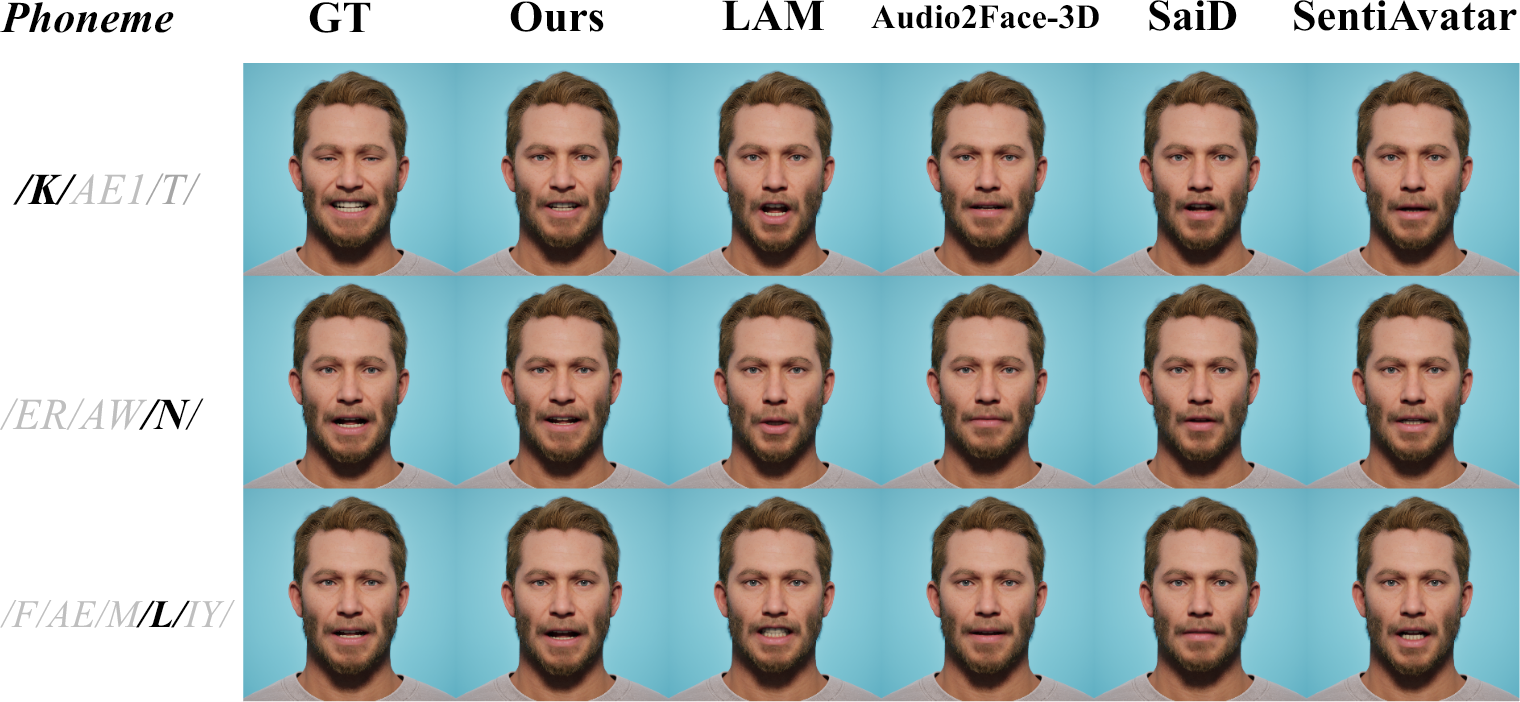
\includegraphics[width=1\linewidth]{comparison.png}
    \caption{
    Qualitative comparison of audio-driven facial animation results.
    From top to bottom, the rows show examples from the words ``cat'', ``around'', and ``family'', respectively.
    The leftmost column shows phoneme annotations, with the active phoneme highlighted in bold black and the surrounding phonemes shown in gray.
    }
    \label{fig:comparison}
\end{figure*}

In this section, we evaluate the proposed language-assisted Audio2ARKit framework through quantitative and qualitative experiments.
We first introduce the dataset used for training and evaluation.
We then describe the experimental setup, including baselines, evaluation metrics, and implementation details.
Next, we compare our method with existing approaches.
Finally, to analyze the contribution of each design component, we conduct ablation studies.


\subsection{Dataset}
\label{subsect:dataset}

We use selected data from BEAT~\cite{liu2022beat} for training and evaluation.

\paragraph{Data Split.}
We use a subject-disjoint split of 277 sequences into 176 training, 40 validation, and 61 test sequences, keeping test speakers unseen during training.
Semantic segmentation yields 21,513 segments: 15,655 for training, 2,858 for validation, and 3,000 for testing.

\subsection{Experimental Setup}
\label{subsect:experimental_setup}

\paragraph{Baselines.}
We compare with SAiD~\cite{park2023said}, Audio2Face-3D~\cite{chung2025audio2face}, LAM-A2E~\cite{lam}, and SentiAvatar~\cite{jin2026sentiavatar}.
Audio2Face-3D, LAM-A2E, and SentiAvatar use their publicly released pretrained weights; SAiD is fine-tuned from its public checkpoint on our training split.

\paragraph{Evaluation Metrics.}
We employ five quantitative metrics to comprehensively evaluate the performance: Mean Squared Error (MSE), Mean Absolute Error (MAE), Fréchet Distance (FD), Wasserstein Inception Distance (WInD), and Lip Landmark Distance (LMD). MSE and MAE measure the frame-level accuracy of the predicted ARKit blendshape coefficients against the ground truth. FD evaluates the distributional discrepancy between the predicted motion sequences and the ground-truth sequences in the extracted feature space. WInD, following the protocol introduced in prior work \cite{park2023said}, provides a robust benchmark for comparing the perceptual quality and temporal dynamics of the generated sequences against the ground truth. LMD measures the mean Euclidean distance between detected 2D mouth landmarks in paired rendered videos.

\paragraph{Implementation Details.}
The general preprocessing pipeline combines ASR with SAT~\cite{frohmann2024segment} for transcript extraction and semantic segmentation.
Our generator is initialized from Qwen3-Omni-30B-A3B-Instruct~\cite{xu2025qwen3omni} and adapted with LoRA~\cite{hu2021lora} on the language decoder, with the audio encoder and multimodal alignment modules frozen.
We train SFT and GRPO for four epochs each on four NVIDIA A100 GPUs, with global batch sizes of 8 and 24, respectively.
GRPO combines coefficient, temporal, and mouth-geometry feedback.


% TODO: Document the exact post-processing switches for the reported result groups.
\subsection{Comparison with Audio2ARKit Methods}
\label{sec:main_comparison}

We compare AudioMouth with four competitive baselines: LAM-A2E~\cite{lam}, NVIDIA Audio2Face-3D~\cite{chung2025audio2face}, SAiD~\cite{park2023said}, and SentiAvatar~\cite{jin2026sentiavatar}. To ensure fair comparison, we extract speaking segments from both ground-truth and generated sequences based on the script and concatenate them, since our method focuses specifically on speech-related mouth motion prediction.

Predictions are concatenated and post-processed as described in Section~\ref{sec:stage3}. In the tables, SFT denotes the generator in the second stage and Refined (GRPO) denotes the generator after refinement; both use the reported post-processing setting.

\begin{table}[t]
\centering
{\fontsize{9}{10.5}\selectfont
\renewcommand{\arraystretch}{1.02}
\begin{tabular*}{\textwidth}{
    @{\extracolsep{\fill}} lccccc @{}
}
\hline
\textbf{Methods}
& \textbf{MSE $\downarrow$}
& \textbf{MAE $\downarrow$}
& \textbf{FD $\downarrow$}
& \textbf{WInD $\downarrow$}
& \textbf{LMD $\downarrow$} \\
\hline

LAM-A2E
& $0.023$
& $0.109$
& $38.403 \pm 10.149$
& $41.751 \pm 10.885$
& $7.648 \pm 0.497$ \\

Audio2Face-3D
& $0.020$
& $0.106$
& $25.228 \pm 3.560$
& $29.879 \pm 4.454$
& $7.879 \pm 0.438$ \\

SAiD
& $0.021$
& $0.108$
& $58.357 \pm 21.580$
& $62.256 \pm 21.911$
& $7.651 \pm 0.504$ \\

SentiAvatar
& $0.022$
& $0.106$
& $40.609 \pm 10.277$
& $42.153 \pm 10.542$
& $8.131 \pm 1.005$ \\

AudioMouth
& $\mathbf{0.006}$
& $\mathbf{0.053}$
& $\mathbf{10.820 \pm 2.635}$
& $\mathbf{16.513 \pm 3.584}$
& $\mathbf{6.249 \pm 0.723}$ \\
\hline
\end{tabular*}
}
\caption{Comparison with Audio2ARKit methods on 60 scripts from the selected test data. AudioMouth is the generator after Sequence-Level Motion Refinement with post-processing. FD, WInD, and LMD are mean $\pm$ sample standard deviation across scripts. Bold indicates the lowest reported value in each column.}
\label{tab:quantitative_results}
\end{table}

% Original table retained for reference; the figure is used in the compiled manuscript.
% \begin{table}[t]
% \centering
% {\fontsize{9}{10.5}\selectfont
% \renewcommand{\arraystretch}{1.02}
% \begin{tabular*}{\textwidth}{@{\extracolsep{\fill}} lccccc @{}}
% \multicolumn{6}{c}{\textbf{(a) Linguistic and Articulatory Conditioning}} \\[0.15em]
% \hline
% \textbf{Methods}
% & \textbf{MSE $\downarrow$}
% & \textbf{MAE $\downarrow$}
% & \textbf{FD $\downarrow$}
% & \textbf{WInD $\downarrow$}
% & \textbf{LMD $\downarrow$} \\
% \hline
%
% w/o Guidance
% & $0.007484$
% & $0.057885$
% & $53.743 \pm 74.384$
% & $62.356 \pm 76.296$
% & $6.917 \pm 0.818$ \\
%
% Audio Only
% & $0.007288$
% & $0.059896$
% & $83.640 \pm 94.524$
% & $93.230 \pm 96.674$
% & $6.938 \pm 0.989$ \\
%
% SFT
% & $\mathbf{0.005978}$
% & $\mathbf{0.053467}$
% & $\mathbf{11.282 \pm 3.888}$
% & $\mathbf{17.052 \pm 4.990}$
% & $\mathbf{6.297 \pm 0.825}$ \\
% \hline
% \end{tabular*}
%
% \vspace{0.5em}
%
% \begin{tabular*}{\textwidth}{@{\extracolsep{\fill}} lccccc @{}}
% \multicolumn{6}{c}{\textbf{(b) Distribution-Balanced Supervision}} \\[0.15em]
% \hline
% \textbf{Methods}
% & \textbf{MSE $\downarrow$}
% & \textbf{MAE $\downarrow$}
% & \textbf{FD $\downarrow$}
% & \textbf{WInD $\downarrow$}
% & \textbf{LMD $\downarrow$} \\
% \hline
%
% w/o Reweighting
% & $0.012226$
% & $0.074727$
% & $21.663 \pm 8.109$
% & $29.253 \pm 7.603$
% & $9.011 \pm 0.630$ \\
%
% SFT
% & $\mathbf{0.005978}$
% & $\mathbf{0.053467}$
% & $\mathbf{11.282 \pm 3.888}$
% & $\mathbf{17.052 \pm 4.990}$
% & $\mathbf{6.297 \pm 0.825}$ \\
% \hline
% \end{tabular*}
%
% \vspace{0.5em}
%
% \begin{tabular*}{\textwidth}{@{\extracolsep{\fill}} lccccc @{}}
% \multicolumn{6}{c}{\textbf{(c) Motion Refinement and Geometric Feedback}} \\[0.15em]
% \hline
% \textbf{Methods}
% & \textbf{MSE $\downarrow$}
% & \textbf{MAE $\downarrow$}
% & \textbf{FD $\downarrow$}
% & \textbf{WInD $\downarrow$}
% & \textbf{LMD $\downarrow$} \\
% \hline
%
% SFT
% & $0.005978$
% & $0.053467$
% & $11.282 \pm 3.888$
% & $17.052 \pm 4.990$
% & $6.297 \pm 0.825$ \\
%
% w/o SLMD
% & $0.006003$
% & $0.053598$
% & $14.268 \pm 24.299$
% & $20.211 \pm 25.147$
% & $6.341 \pm 0.783$ \\
%
% Refined (GRPO)
% & $\mathbf{0.005713}$
% & $\mathbf{0.052878}$
% & $\mathbf{10.820 \pm 2.635}$
% & $\mathbf{16.513 \pm 3.584}$
% & $\mathbf{6.249 \pm 0.723}$ \\
% \hline
% \end{tabular*}
% }
% \caption{Ablations of complementary supervision on 60 scripts from the selected test data. (a) Linguistic and articulatory conditioning during SFT. (b) SFT with and without coefficient-value reweighting. (c) Sequence-level refinement and its geometric reward component. All variants use the reported post-processing setting. ``w/o Reweighting'' assigns unit weights to coefficient-value tokens; ``w/o SLMD'' removes the simplified 3D geometric reward. FD, WInD, and LMD are mean $\pm$ sample standard deviation across scripts. Bold marks the lowest reported value in each panel.}
% \label{tab:ablations}
% \end{table}


Quantitatively, Table~\ref{tab:quantitative_results} compares the complete framework with four baselines on the same selected test data. AudioMouth has the lowest values in all five columns. MSE is $0.006$, compared with the best baseline value of $0.020$; FD is $10.820$ versus $25.228$, and LMD is $6.249$ versus $7.648$. Together with lower MAE and WInD, these results support lower coefficient error, closer motion distributions in the feature space, and lower rendered lip-landmark error. They do not directly establish synchronization or perceptual naturalness.

Qualitatively, Figure~\ref{fig:comparison} compares representative mouth shapes for ``cat'', ``around'', and ``family'' with the corresponding ground truth. The phoneme annotations in the leftmost column identify the speech sounds associated with the displayed frames. These examples illustrate differences in lip closure and mouth opening and complement the coefficient and landmark comparisons.

\begin{figure}[!htbp]
    \centering
    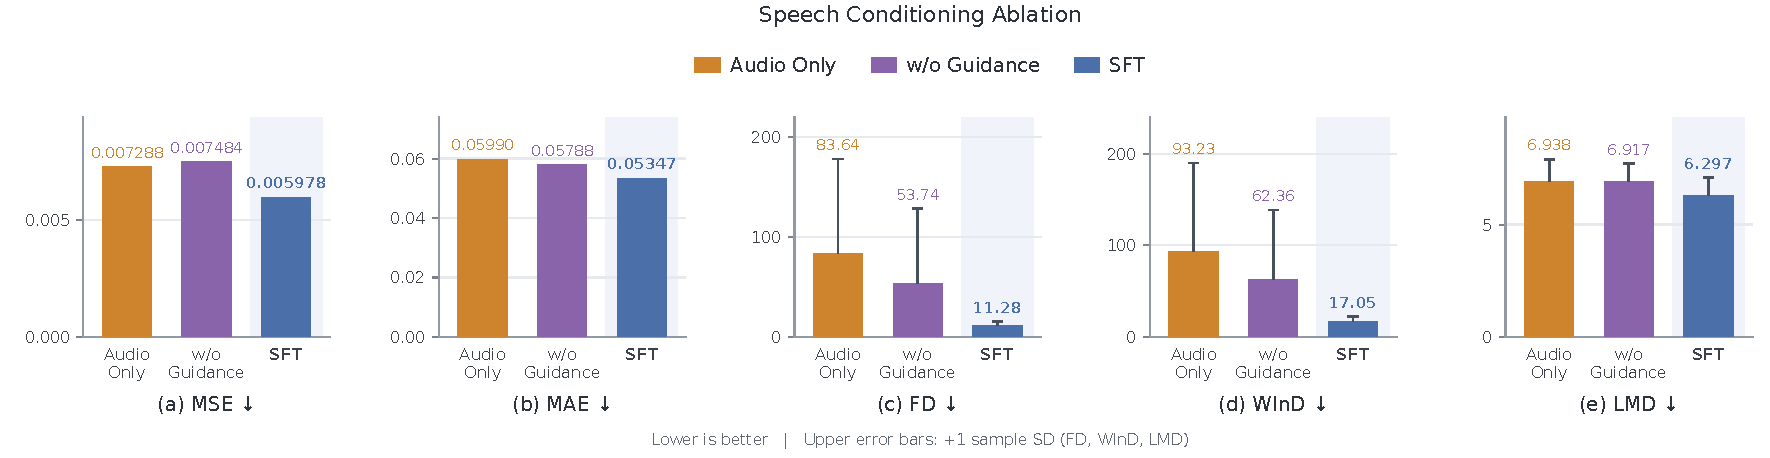
\includegraphics[width=\linewidth]{figures/ablation_conditioning_wide.pdf}
    \caption{Speech conditioning ablation. From left to right, we compare Audio Only, w/o Guidance, and the full SFT model. Results use 60 scripts from the selected test data. SFT is blue and GRPO is teal wherever shown. Lower values are better. Upper error bars show one sample standard deviation for FD, WInD, and LMD; MSE and MAE are aggregate values.}
    \label{fig:ablation_conditioning}
\end{figure}


\noindent\textbf{Ablation of Linguistic and Articulatory Conditioning.}
To examine the role of explicit linguistic inputs, we compare the full SFT generator with two variants: w/o Guidance removes articulation instructions while retaining transcripts and phonemes, and Audio Only removes all three while using the same segmented audio (Figure~\ref{fig:ablation_conditioning}).
Full conditioning gives the best overall coefficient accuracy, distributional agreement, and lip-landmark accuracy among these variants.
The two comparisons assess the contribution of articulation guidance and the joint contribution of transcript and phoneme inputs.
A plausible explanation is that linguistic cues expose speech structure, while articulation instructions connect that structure to the named facial controls, reducing the ambiguity the generator must resolve from acoustics alone.
Together, these results support conditioning structured motion generation on both linguistic content and explicit articulatory relations.

\begin{figure}[!htbp]
    \centering
    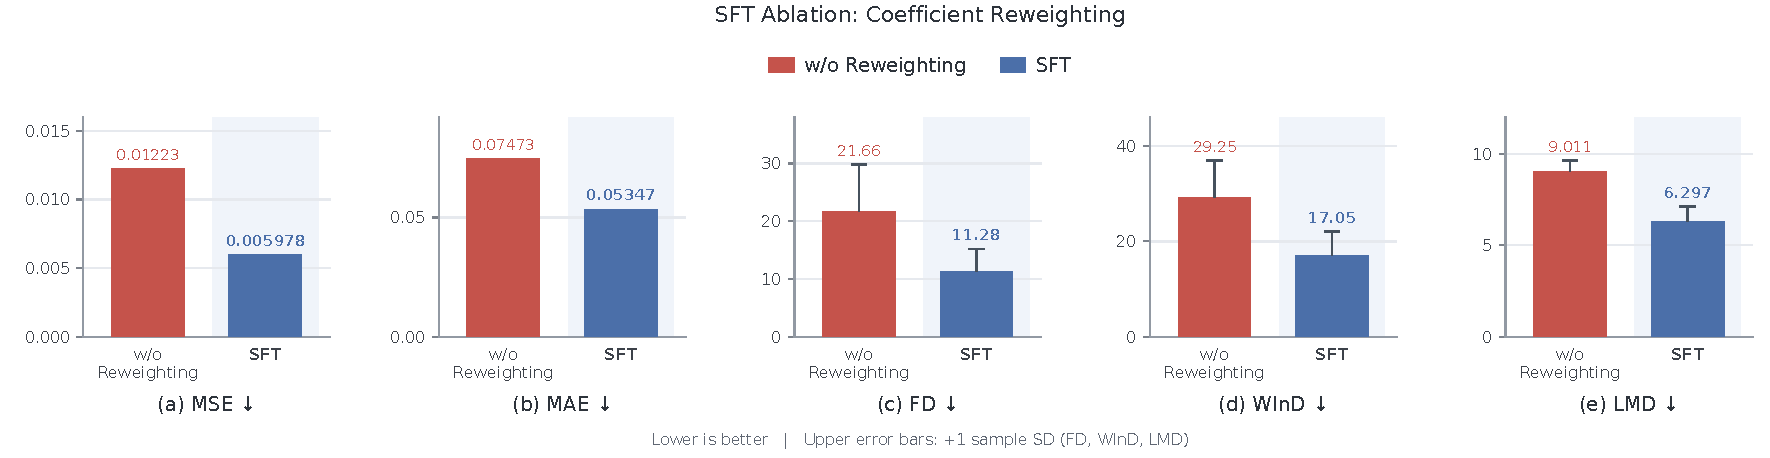
\includegraphics[width=\linewidth]{figures/ablation_reweighting_wide.pdf}
    \caption{SFT ablation of distribution-balanced supervision. The SFT model is compared with a variant using unit weights for coefficient-value tokens, with the same conditioning and post-processing. Results use 60 scripts from the selected test data. SFT is blue and GRPO is teal wherever shown. Lower values are better. Upper error bars show one sample standard deviation for FD, WInD, and LMD; MSE and MAE are aggregate values.}
    \label{fig:ablation_reweighting}
\end{figure}


\noindent\textbf{Ablation of Distribution-Balanced Supervision.}
To assess the effect of coefficient-value imbalance, we compare the weighted SFT objective with w/o Reweighting, which assigns unit weight to coefficient-value tokens while retaining the same conditioning and post-processing (Figure~\ref{fig:ablation_reweighting}).
Reweighting improves all five reported metrics, indicating benefits for both coefficient reconstruction and the resulting motion distribution and mouth shape.
This comparison evaluates the contribution of the supervised objective independently of adding linguistic inputs or GRPO refinement.
Downweighting frequent low-valued targets reduces their dominance in the loss and gives larger coefficient values greater relative emphasis during training.
The observed gains are consistent with this motivation and support distribution-balanced supervision for structured coefficient generation.

\begin{figure}[!htbp]
    \centering
    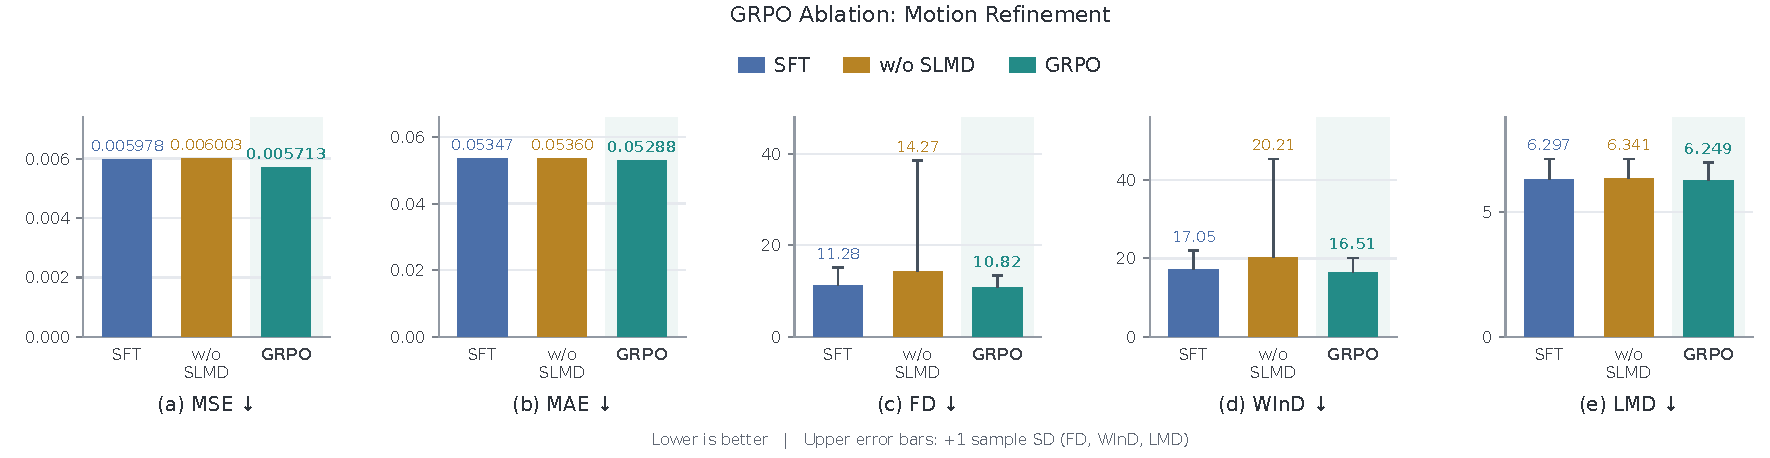
\includegraphics[width=\linewidth]{figures/ablation_motion_wide.pdf}
    \caption{GRPO ablation of motion refinement and geometric feedback. We compare SFT, GRPO refinement without SLMD, and the full refined generator under the same post-processing setting. Results use 60 scripts from the selected test data. SFT is blue and GRPO is teal wherever shown. Lower values are better. Upper error bars show one sample standard deviation for FD, WInD, and LMD; MSE and MAE are aggregate values.}
    \label{fig:ablation_motion}
\end{figure}


\noindent\textbf{Ablation of Sequence-Level Motion Refinement beyond SFT.}
To evaluate whether motion-level feedback complements token-level learning, we compare the SFT generator with Refined (GRPO) under the same post-processing setting (Figure~\ref{fig:ablation_motion}).
Refinement yields modest, consistent improvements in coefficient accuracy, distributional agreement, and lip-landmark accuracy.
This comparison assesses the additional value of sequence-level optimization after supervised adaptation.
The pattern is consistent with the reward supplying feedback on the decoded trajectory's dynamics and geometric effects, which next-token likelihood does not directly measure.
These results support using motion-aware refinement to complement the structured generation learned during SFT.

\noindent\textbf{Ablation of Explicit Geometric Mouth-Motion Feedback.}
To assess the contribution of geometric feedback within refinement, we compare the full reward with w/o SLMD, which omits the simplified 3D lip-geometry term (Figure~\ref{fig:ablation_motion}).
The full reward achieves lower mean errors across all reported metrics, whereas removing SLMD also loses the distributional gains over SFT.
This comparison examines the value of geometric supervision alongside coefficient and temporal discrepancies.
The improvement is consistent with SLMD coupling multiple controls through their combined effect on mouth deformation, a relationship that coefficient-wise errors do not represent explicitly.
The results therefore support the inclusion of geometric feedback in the refinement objective.
